%!TEX root = ../paper.tex

%\newcommand{\dims}[1]{\langle #1 \rangle}

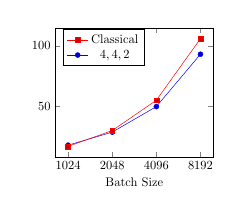
\begin{tikzpicture}[scale=.45]
    \begin{axis}[
        width=.5\textwidth,
        xmode=log,
        log basis x={2},
        xlabel=Batch Size, 
        %ylabel=Per-batch training time in seconds,
        legend style={at={(.05,.85)},anchor=west},
        xtick={1024,2048,4096,8192},
        xticklabels={1024,2048,4096,8192},
            /pgf/number format/.cd, 1000 sep={},
            reverse legend,
    ]
    \addplot 
    coordinates {(8192,93.19120597839355) (4096,49.998961210250854)
    (2048,28.92702865600586) (1024,18.19733500480652)};
    \addplot 
        coordinates {(8192,106.00743579864502) (4096,55.22960305213928) 
            (2048,30.237940549850464) (1024,17.160202264785767)};
    \legend{$\dims{4,4,2}$,Classical}
    \end{axis}
\end{tikzpicture}